\subsection{Session page}
To create a session the user must first reach the Sessions component, which can be accessed through the “Sessions” button on the navbar. The session page has the URL /admin/sessions. A session cannot be created until both a course and a question are present in the database. Therefore, the user should visit both the dashboard and the question page, before accessing the session page. The figure \ref{fig:sessionPage} shows the session page, in this figure 2 sessions has already been created called “Test Økt” and “TestØkt2”. Since there is a session in the database. 

The Session component is visible in the Sessions component on the right side of the page. The Session component contains a search bar and a select box identical to the ones on the question page. The component also contains a list that includes all the current sessions for the chosen subject. Like in the list on the question page, the list on the session page must send a socket emit message to the server in order to keep its session list updated. The list is updated whenever the Session component is loaded, a new session is created, or whenever the chosen course is changed. If there are no sessions for the chosen course, then only the Sessions component is displayed on the page. Although if this is the case, then the Sessions component is not going to have any sessions in the list.
\\[11pt]
Once the Session component is visible, the information displayed on the component varies depending on the current question being selected. The user can easily change between the available sessions and their questions by clicking on them. On figure \ref{fig:sessionPage} you can see that the session “Test Økt” has opened the question “Text Question”. 
\\[11pt]
The information displayed on the Session component comes from a component by the name DisplayQuestion. The DisplayQuestion is a component that is used whenever an admin is going to watch question information in the same style as it would look in an active session. Essentially the component is used on the session page and on the user profile page. The DisplayQuestion component uses a vue-card, which makes it easier to toggle between showing the question information or the question's solution. There is a component for the answer object and a component for the solution object for each question type in the DisplayQuestion component. Only one of these components can be used at a time. The DisplayQuestion component must accommodate for the fact that some of the question types require the GraphDrawer to visually display their solution object. The DisplayQuestion component needs to display the shown question’s type. This is done to avoid confusing users with certain question types, as some of the question types have similar format for the GraphDrawer.
\begin{figure}[H]
	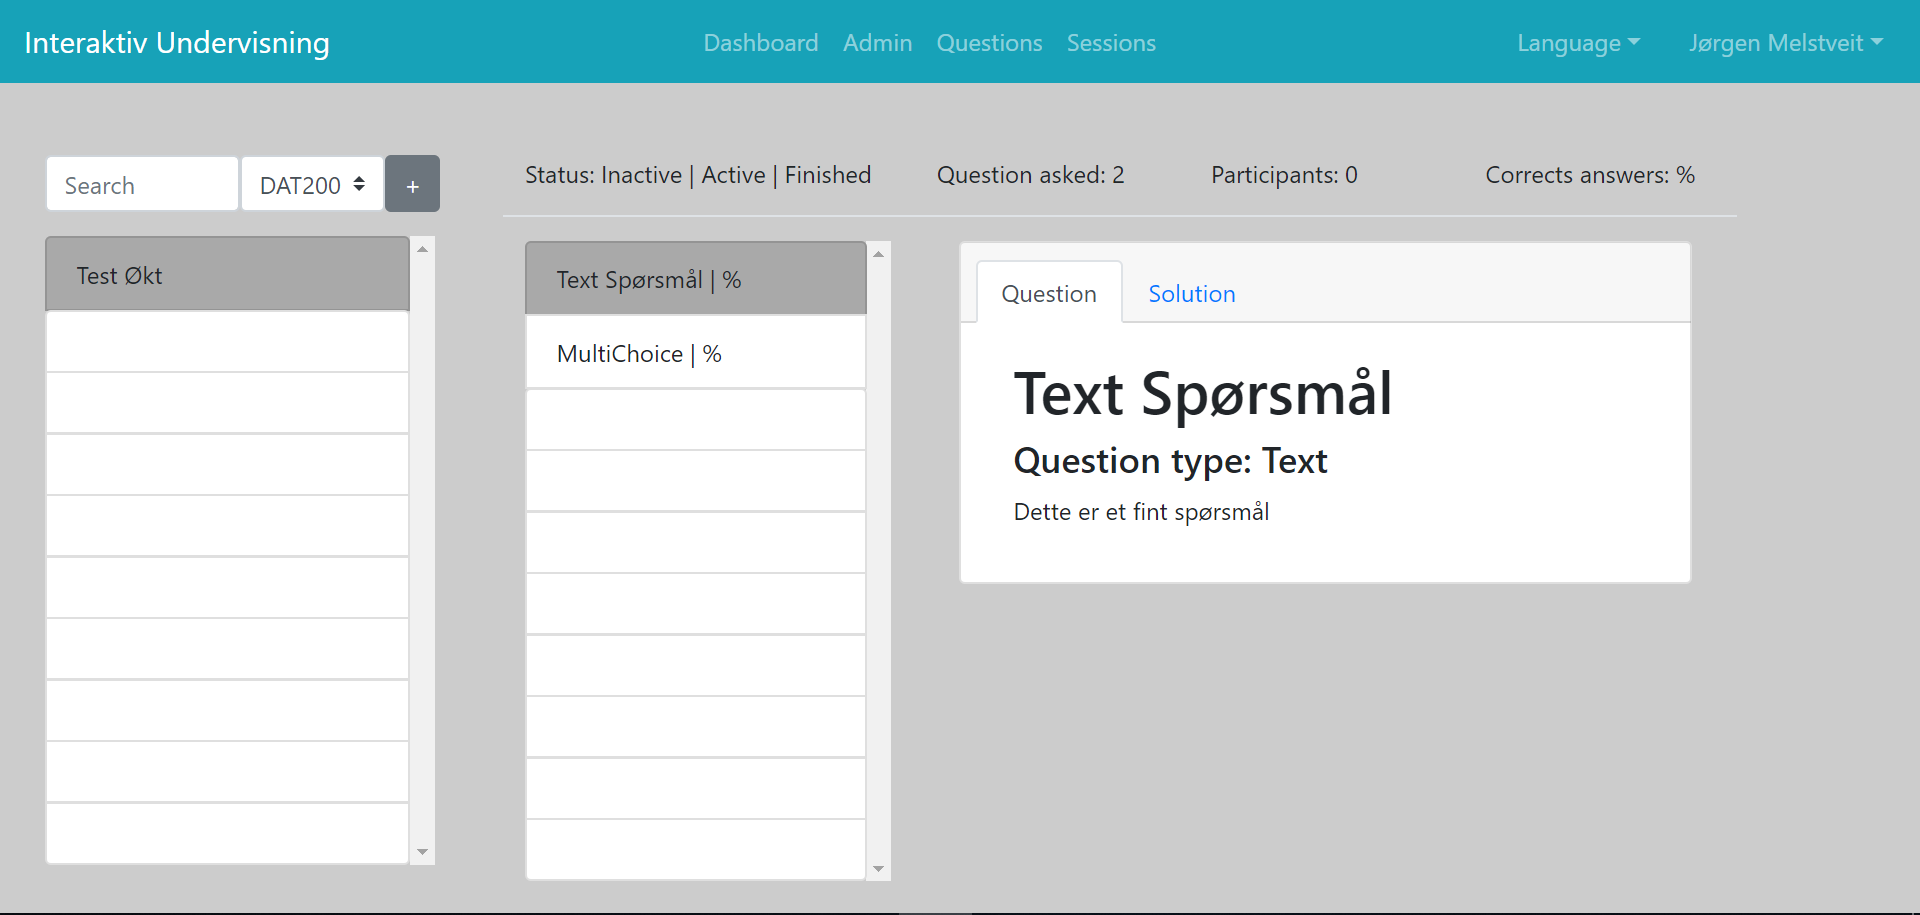
\includegraphics[width=0.80\linewidth]{sessionPage}
	\caption{This figure display the session page. In the image the user is currently checking out the session Test Økt. The Session and DisplayQuestion components are both visible to the right of the image. Currently the Text Spørsmål is selected and the DisplayQuestion is showing its basic information. Such as the title, description and question type.}
	\label{fig:sessionPage}
\end{figure}
\noindent
To create a new session, the EditSession component must first be opened. This is done by having the user click on the button with the “+” label. 
This component displays all the available questions of the chosen course using a vue-modal. Like the EditQuestion component, the EditSession component has a data object called newSession. This object should have all the values needed for the server to create a new session and add it to the database. The current course should have already been chosen at this point, therefore the course variable in the newSession object have been assigned with this course value. This value is used by EditSession component whenever it sends a socket emit to the server, asking the server for all the questions in the given course. The EditSession component allows the user to give the session a title and add a question to the session. Once a user has chosen one of the questions, the question is added to the questions array in the newSession object. The content of the questions array is displayed on the EditSession component under the previous list, and it reacts to any changes done to the array. This is noticeable in the figure \ref{fig:editSessionComponent}, where you can see the Text Question has been added to the list under the questions list. Once a question is visible in this way, it means the question is a part of the newly created session. Of course, nothing is stored on the server until the user has confirmed its changes with the button labeled “Ok”. When the button is pressed the EditQuestion sends a socket emit with the newSession object to the server. The server collects the objects and the information is used to insert a new session into the Session database table. Afterwards all the questions in the questions array are linked to the session in another database table in between the Session and Questions tables called the SessionsHasQuestion. When everything is done the server sends a emit response back to the client. The EditSession component should be closed and the Sessions component reacts to the emit response by sending a new socket emit back to the server, in order to update its session list. Once the server responds with the updated session content, the list on the Session component should include the newly created session.  
\begin{figure}[H]
	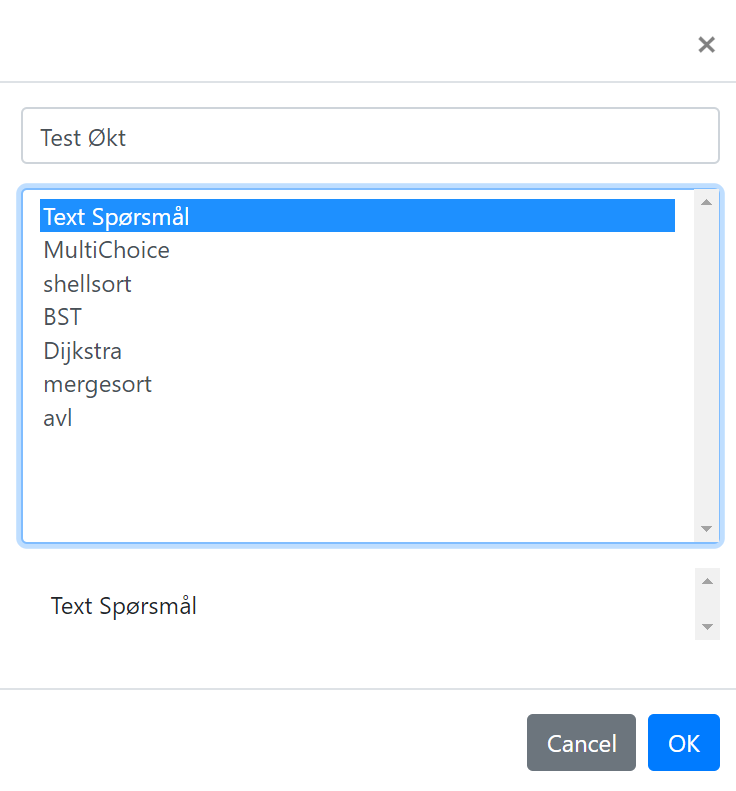
\includegraphics[width=0.80\linewidth]{createANewSession}
	\caption{This figure displays an image of the EditSession component. In the image the user is planning on creating a new session by the name of Text Økt. The image also shows the user having clicked on the Text Spørsmål, which now have been added to the list at the bottom of the page.}
	\label{fig:editSessionComponent}
\end{figure}
\noindent
It is also possible to edit or delete existing sessions, but only if their status is set to “Inactive”. The sessions status is visible on the Session component, where the current session status is the status that is visibly underlined. The status will remain “Inactive” as long as its not initialized. When an admin or student assistant starts a waiting room for a session. The status changes to “Active”, and it is no longer possible to edit or delete this session. Once a session is finished and all the questions have been answered, the status is changed to “Finished”. If an admin user or student assistant decides to use this session again, then the status is changed back to “Active” again until the session is finished. The reason for not allowing any users to edit or delete active sessions are the same for not allowing users the ability to edit or delete questions once they’ve been assigned to a session. Deleting or editing a session after use would affect the previous session results for both the teacher and students. If the status is no longer “Inactive” the background color to the edit and delete buttons are changed to grey. This is an indication that these buttons are no longer to be used. If a user still tries to click on the buttons, the user is informed that it is no longer possible to use this functionality. Using the edit functionality works a lot like it did for the editing questions. The EditQuestion component is again used, but all the data previously saved for the chosen session are filled in the component. Any changes done to the session won’t apply until the user confirms his action using the button labelled “OK”. On the server side, the server does not check for validation or create any solutions which are only used for adding/editing questions. It instead goes directly to using the SQL command update for updating an existing session in the database or the insert command the inserting a new session into the database. Removing a session simply sends a socket emit to the server asking the server to delete the chosen session from the database. After the session is deleted from the database, the list in the Sessions component is updated again, and the chosen session should no longer be visible on the page.

